\section{Aufbau und Durchführung}
\label{sec:auf_durch}

Im Folgenden wird der Aufbau und die Durchführung des versuchs beschrieben.

\subsection{Der Aufbau}
\label{sec:aufbau}

Die Materialien für den Versuch sind in Abbildung \ref{fig:material} zu sehen. Für den Versuch stehen in einem Baukasten kugelförmige Hohlraumresonatoren als Halbkugeln mit Lautsprecher und Mikrofon jeweils in einer der beiden Hälften. Außerdem gibt es 2 weitere Halbkugeln mit einem Loch und dazugehörige Blenden mit den Durchmessern von $d = \{ 10, 13, 16 \} \, \mathrm{mm}$. Zusätzlich sind in einem Baukasten zylinderförmige Hohlraumresonatoren mit den Längen von $h = \{12.5, 50, 75\} \, \mathrm{mm}$ und Blenden mit den Durchmessern von $d = \{ 10, 13, 16 \} \, \mathrm{mm}$ vorhanden. Diese Bauteile können auf eine Schiene aufgebracht werden, wo dann auch ein Lautsprecher und ein Mikrofon als Enden vorhanden sind. Die Messung kann einerseits über einen Computer mit der Software namens \textit{SpectrumSLC} durchgeführt werden. Dabei bietet die Schnittstelle mit dem Computer ein Audiosignal an den Lautsprecher und aknn die Signale des Mikrofons empfangen und verarbeiten. Eine andere Variante ist die Messung mit Hilfe eines Oszilloskops. Die Schaltung ist in Abbildung \ref{fig:schaltung} skizziert. Dafür wird der Lautsprecher an der Steuerelektronik an \textit{Speaker Out} und das Mikrofon an \textit{Micro Input} angeschlossen. Ein Sinusgenerator wird einerseits mit Channel 1 vom Oszilloskop verbunden als auch in \textit{Sine Input} der Steuerelektronik. Channel 2 wird an den Anschluss namens \textit{AC Monitor} in der Steuerelektronik angeschlossen. in der Steuerelektronik ist ein Frequenz-Amplitude-Konverter vorhanden, damit die Frequenzen am Oszilloskop untersucht werden können. Mit Hilfe der sweep-Funktion des Sinusgenerators können dann die Daten zeitlich mit der Frequenz am Oszilloskop verarbeitet werden. Am PC können die Daten direkt gespeichert werden udn am Oszilloskop können durch Anschließen eines USB-Sticks die Bilder gespeichert werden.

\begin{figure}[H]
    \centering
    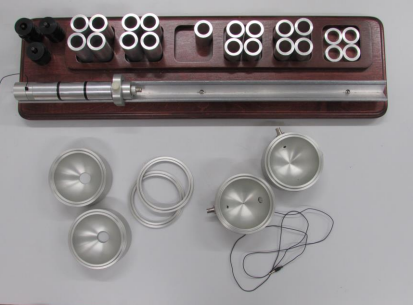
\includegraphics[width=0.8\textwidth]{build/Experiment.PNG}
    \caption{Hohlraumresonatoren und Irisblenden. \cite{Anleitung}}
    \label{fig:material}
\end{figure}

\begin{figure}[H]
    \centering
    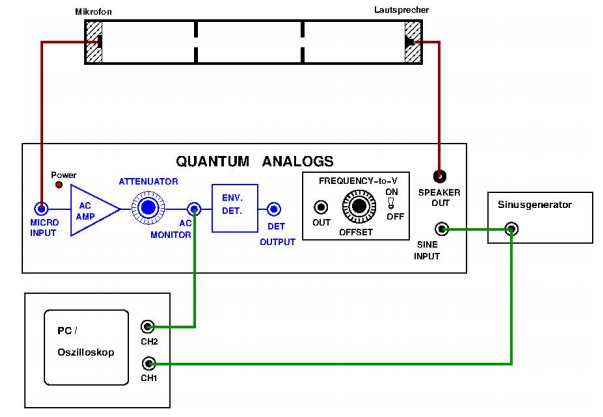
\includegraphics[width=0.8\textwidth]{build/Schaltung.PNG}
    \caption{Skizze der Schaltung des Versuchs. \cite{Anleitung}}
    \label{fig:schaltung}
\end{figure}

\subsection{Vorbereitende Experimente}
\label{sec:vorbereitung}

Bevor mit den richtigen Experimenten angefangen werden kann, muss die Versuchstechnik getestet werden. Dafür werden die zylinder mit einer Länge von $50 \, \mathrm{mm}$ benötigt. Es wird nun zuerst ein Zylinder Zwischen Lautsprecher und Mikrofon gestellt und ein Frequenzspektrum von $100 \, \mathrm{Hz}$ bis $12 \, \mathrm{kHz}$ mit dem Oszilloskop aufgenommen und dokumentiert. Danach wird ein Zylinder an die Kette angehangen und das selbe Spektrum aufgenommen. Dies wird bis zum 12. Zylinder durchgeführt. Danach wird die selbe Messung mit dem Computer durchgeführt. Die Frequenzspektren sollten jeweils keine signifikanten Unterschiede zwischen der Messung mit dem Oszilloskopund dem Computeraufweisen. Zum Schluss wird ein Frequenzspektrum eines einzelnen $75 \, \mathrm{mm}$ Zylinders mit Oszilloskop und Computer aufgenommen und verglichen.

\subsection{Das Wasserstoffatom}
\label{sec:d_H}



\subsection{Das Wasserstoffmolekül}
\label{sec:d_H2}



\subsection{Der 1-dim Festkörper}
\label{sec:d_fk}